\chapter{Vorgehen Performance Analyse}
\section{Motivation}

Die Performance respektive Leistungsfähigkeit einer Applikation stellt einer der bedeutendsten Qualitätsanforderungen dar. Sie kann bei den Benutzern nicht nur zur Verärgerung, sondern auch zu einer Verlangsamung der Business-Prozesse führen. Die Motivation für eine Performance-Analyse entsteht, wenn die in Service Level Agreement oder Anforderungsanalyse spezifizierten \textbf{Qualitätsanforderungen nicht erfüllt} sind. Optimalerweise ist die Überprüfung dieser Anforderungen Bestandteil ein jedes Software Entwicklungszyklus respektive des (automatisierten) Testprozesses.

\section{Ablauf}
Die Performance-Analyse ist grundsätzlich ein iterativer Prozess und so lange bis die Anforderungen und der Kunde zufrieden sind. Sie besteht aus folgenden vier Schritten\cite{hummelBeer201109}:
\begin{enumerate}
	\item Identifikation der neuralgischen Punkte des Systems
	\item \textbf{Suche nach dem Dominating Consumer\footnote{Kirk Pepperdine bezeichnet die Aktivität, welche dominiert wie die CPU gebraucht wird, als Dominating Consumer . }}
	\item \textbf{Sammeln von Detaildaten}
	\item Lösen des Problems
\end{enumerate}

Punkt zwei und drei sind weiter unten weiter beschrieben.

\section{Suche nach dem Dominating Consumer}\label{dominating_consumer}
Die Suche nach dem Dominating Consumer kann nach folgendem strukturierten Schema gemacht werden:
\begin{figure}[H]
  	\centering
    	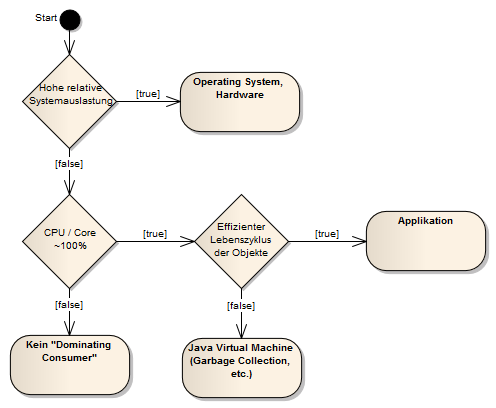
\includegraphics[width=13.1cm]{images/dominating_consumer}
        	\caption{Suche nach dem Dominating Consumer}
\end{figure}

\subsection{Hohe relative Systemauslastung}\label{hohe_systemauslastung}
Die erste Frage, die sich bei der Suche nach dem Dominating Consumer stellt ist, ob die Hohe CPU-Auslastung\footnote{CPU kann auch einer oder ein paar Cores bedeuten.} durch das System respektive den Kernel verursacht wird. Unter den verschiedenen Betriebssystemen gibt es verschiedene Werkzeuge, um dies herauszufinden:
\begin{itemize}
	\item \textbf{Windows:} Auf der Lasche Performance (Leistung) des Task Managers. Es muss dafür via View / Show Kernel Times allerdings noch die Kernelzeit eingeblendet werden.
	\item \textbf{Linux / Unix: } vmstat zeigt die Ausnutzung der CPU: vmstat 5
\end{itemize}

Hohe Systemauslastung kann unterschiedliche Gründe haben: 
\begin{itemize}
\item \textbf{Exzessive Context-Switch\footnote{Kontextwechsel}:} Mehrere Prozesse können sich die gleiche CPU (CPU-Kern) nur teilen, wenn beim Wechsel von Prozess A auf B ein Context-Switch gemacht werden kann, so dass Thread B am selben Ort weiterarbeiten kann wie vorher. Gründe für exzessives Context-Switching können beispielsweise nicht adäquat gewählte Locks sein. Wenn ein Thread aufgrund der Synchronisation angehalten werden muss.\footnote{Beispielsweise wenn vmstat berichtet, dass das System nicht im Leerlauf ist, aber die Kernelzeiten (cpu/sy) trotzdem die Zeit des Benutzers (cpu/us) dominiert.}
\item \textbf{Hohe I/O Festplatte} 
\item \textbf{Hohe I/O Netzwerk} 
\end{itemize}


\subsection{Hohe CPU- respektive Core-Last}
Sofern die im Abschnitt \titleref{hohe_systemauslastung} beschriebenen Punkte nicht zutreffen, stellt sich die Frage, ob die Auslastung der CPU überhaupt gross ist. Ist das nämlich nicht der Fall, stehen die Chancen Gut, dass es gar keinen Dominating Consumer gibt. Wenn es keinen Dominating Consumer gibt stellt sich die Frage, was die Threads weg von der CPU halten. Dafür gibt es laut \cite{pepperdine201102} unterschiedliche Gründe:
\begin{itemize}
\item \textbf{Dead Locks: } Threads schliessen sich gegenseitig aus. 
\item \textbf{Applikation skaliert nicht: } Applikation hat schlechte multi-core Eigenschaften.
\item \textbf{Langsame Disks / Netzwerke}
\item \textbf{Zu kleine Connection- und Thread-Pools}
\item \textbf{Aurufe auf langsame externe Systeme}
\end{itemize}


\subsection{Effizienter Objekt-Lebenszyklus}
Sofern die relative Systemlast klein ist und die CPU-Auslastung trotzdem gross ist, muss der Lebenszyklus der Objekte angeschaut werden. Dies kann auf unterschiedliche Arten getan werden:
\begin{itemize}
\item \textbf{Memory Analyse: }Es wird angeschaut, wie alt die Objekte in den verschiedenen Bereiche (Young Collection, Old Collection) sind. 
\item \textbf{Garbage Collection: }Wann und wie oft werden Garbage Collections durchgeführt, wie lange haben sie gedauert, wieviel Speicher haben sie befreit.
\end{itemize}

\section{Sammeln von Detaildaten}
Je nachdem welches der Dominating Consumer ist, müssen weitere Daten gesammelt werden oder andere Analysen gemacht werden. Die folgenden beiden Abschnitte gehen tiefer in die Grundlagen der Garbage Collection und zeigen auch die Eigenheiten der JRockit Virtual Machine.


